% !TeX root = ../main.tex
% !TeX encoding = UTF-8
% !TeX spellcheck = none

\section{Methodology}\label{sec:methodology}

\subsection{Overall Framework}\label{sec:framework}

Figure~\ref{fig:rbsrn-architecture} shows the overall architecture of RBSRN. The framework first generates a base prediction through shared dual-frequency spatiotemporal encoding. The State-Evidence Expert Residual Refinement Module (SERR) organizes correction evidence through self-evolution and directed time-lagged experts. Background-conditioned Cross-region Message Selection (BCMS) selects cross-region historical messages according to source and target traffic backgrounds and the forecast horizon. The two modules read the shared representations in parallel, generate complementary corrections, and combine them additively at the prediction stage:
\begin{equation}
\label{eq:overall-prediction}
\widetilde{Y}=\widetilde{Y}^{0}+\Delta\widetilde{Y}^{S}+\Delta\widetilde{Y}^{B}.
\end{equation}
Here, \(\widetilde{Y}^{0}\) is the base prediction, and \(\Delta\widetilde{Y}^{S}\) and \(\Delta\widetilde{Y}^{B}\) are the SERR and BCMS corrections, respectively. They correspond to \(Y_{\mathrm{Base}}\), \(\Delta\mathrm{State}\), and \(\Delta\mathrm{Message}\) in the figure. All three belong to \(\mathbb{R}^{H\times N\times2}\) and use the scale standardized separately for each flow channel, as indicated by the tilde. Below, we reindex historical positions as \(k=1,\ldots,T\), denote forecast steps by \(h=1,\ldots,H\), and distinguish flow channels using \(c\in\{\mathrm{in},\mathrm{out}\}\).

\begin{figure}[!htbp]
  \centering
  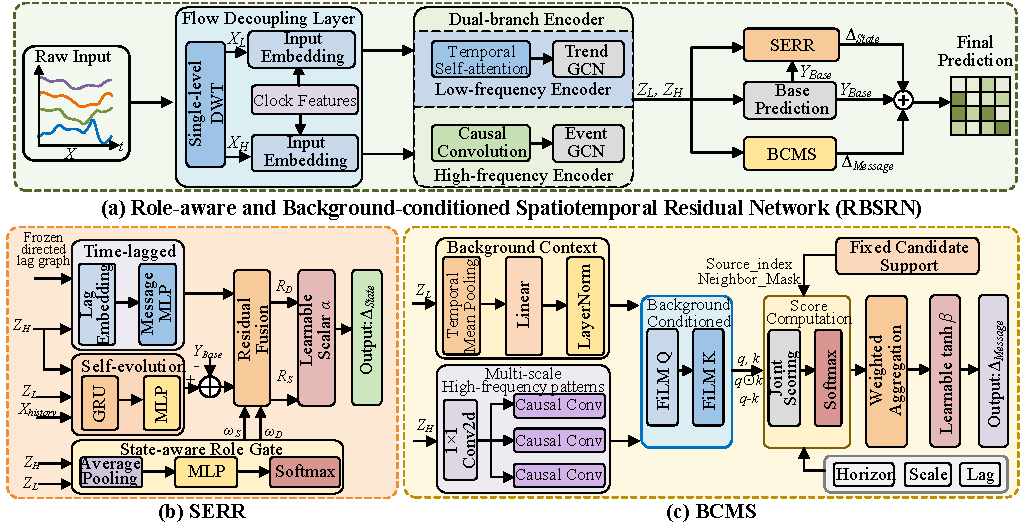
\includegraphics[width=\linewidth]{figures/model-architecture.pdf}
  \caption{\editorialupdated{Overall architecture of RBSRN. (a) Base prediction and parallel residual fusion. (b) SERR expert residual refinement. (c) BCMS background-conditioned historical message selection.}}
  \label{fig:rbsrn-architecture}
\end{figure}

\subsection{Shared Dual-Frequency Spatiotemporal Representations}\label{sec:dual-frequency}

To distinguish smooth changes from short-term fluctuations, RBSRN extracts shared representations through low- and high-frequency branches. We first apply single-level discrete wavelet decomposition and reconstruction along the historical time dimension of each flow channel, producing low- and high-frequency sequences. We standardize both sequences using the channel-wise means and standard deviations of training traffic flow. We then append time-of-day and day-of-week information to obtain \(U_L,U_H\in\mathbb{R}^{T\times N\times4}\). The two branches share the input projection and temporal embeddings. The low-frequency branch applies temporal self-attention and trend graph encoding, whereas the high-frequency branch applies temporal convolution and event graph encoding:
\begin{equation}
\label{eq:low-frequency}
Z_L=\mathrm{F}_L(U_L),
\end{equation}
\begin{equation}
\label{eq:high-frequency}
Z_H=\mathrm{F}_H(U_H),
\end{equation}
where \(Z_L,Z_H\in\mathbb{R}^{T\times N\times d_b}\) and \(d_b\) denotes the shared representation dimension. We fuse the two feature streams using a gated linear unit (GLU) and a rectified linear unit (ReLU) to obtain the base prediction:
\begin{equation}
\label{eq:base-prediction}
\widetilde{Y}^{0}=\mathrm{R}\!\left(\operatorname{ReLU}\!\left[Z_L+\operatorname{GLU}(Z_L)+Z_H\right]\right).
\end{equation}
The convolutional prediction head \(\mathrm{R}\) spans the full historical window and maps the features to inflow and outflow predictions for the next \(H\) steps. SERR and BCMS use \(Z_L\) before the GLU operation, together with \(Z_H\), as their shared inputs.

\subsection{State-Evidence Expert Residual Refinement (SERR)}\label{sec:serr}

SERR organizes two complementary experts around node self-evolution and cross-region time-lagged associations, then allocates their correction contributions according to the current state (Figure~\ref{fig:rbsrn-architecture}(b)). To connect the routine-flow reference with recent dynamics, let \(x_{k,i,c}\) denote the raw flow at historical position \(k\), node \(i\), and channel \(c\). The corresponding routine-flow reference estimated from training data is \(b_{k,i,c}\). We define the state evidence as
\begin{equation}
\label{eq:state-evidence}
\begin{aligned}
\bar{x}_{k,i,c}&=\frac{1}{\ell_k}\sum_{r=k-\ell_k+1}^{k}x_{r,i,c},\qquad \ell_k=\min(3,k),\\
e_{i,c}&=\left[\bar{x}_{T,i,c}-b_{T,i,c},\;x_{T,i,c}-\bar{x}_{T,i,c}\right]^{\mathsf T}.
\end{aligned}
\end{equation}
The two components of \(e_{i,c}\in\mathbb{R}^{2}\) describe trend deviation and short-term fluctuation at the final historical time step, respectively. The mean uses only observed positions within the current historical window and adjusts its length to the available observations at the window's start.

The self-evolution expert encodes recent trajectories within each individual node. For each flow channel, it concatenates the sum of the shared dual-frequency features with raw flow and feeds the result into a shared gated recurrent unit (GRU). It then maps the final hidden state to a multi-step prediction:
\begin{equation}
\label{eq:self-expert}
P^{\mathrm{self}}_{:,i,c}
=\mathcal{P}_{S}\!\left(\psi_S\!\left(\operatorname{GRU}_{\mathrm{last}}
\left([Z_{L,k,i}+Z_{H,k,i}\,\Vert\,x_{k,i,c}]_{k=1}^{T}\right)\right)\right).
\end{equation}
Here, \(\Vert\) denotes feature concatenation, and \(\psi_S\) is a two-layer perceptron with tanh activation. The projection \(\mathcal{P}_S\) linearly maps \(d_b\)-dimensional features to predictions over \(H\) steps. This branch further extracts each node's temporal evolution from the shared spatiotemporal representations.

The directed time-lagged expert retrieves historical features from source nodes through the preconstructed and frozen association set \(\mathcal{E}_c\). For an edge \((j,i,\ell)\in\mathcal{E}_c\), \(j\) is the source node, \(i\) is the target node, and \(\ell\) is a historical lag satisfying \(0<\ell<T\). A lag embedding modulates the source high-frequency features, which are then combined with the target state evidence to form supplementary messages:
\begin{equation}
\label{eq:delay-expert}
\begin{aligned}
\eta_{i,c}&=W_e e_{i,c},\\
m_{j\to i,\ell,c}&=\psi_D\!\left([(1+\tanh v_{\ell})\odot Z_{H,T-\ell,j}\,\Vert\,\eta_{i,c}]\right),\\
R^{\mathrm{delay}}_{:,i,c}&=\mathcal{P}_D\!\left(\eta_{i,c}
+\sum_{(j,i,\ell)\in\mathcal{E}_c}a_{ji\ell}^{c}m_{j\to i,\ell,c}\right).
\end{aligned}
\end{equation}
Here, \(W_e\in\mathbb{R}^{d_b\times2}\) projects the evidence, and \(v_\ell\in\mathbb{R}^{d_b}\) is a learnable lag embedding. The message transformation \(\psi_D\) uses a sigmoid linear unit (SiLU) activation without bias, \(a_{ji\ell}^{c}\) is a fixed edge weight, and \(\mathcal{P}_D\) is a multi-step linear output head. Each expert shares its own parameters across nodes and flow channels, while directed time-lagged associations are specified separately for each flow channel.

A state-conditioned gate determines expert contributions from the temporal means of low- and high-frequency features and the state evidence for both flow channels:
\begin{equation}
\label{eq:role-gate}
\Omega_i=\operatorname{Softmax}_{\mathrm{expert}}\!\left(
\operatorname{reshape}_{2\times2}\,g\!\left(
[\bar{Z}_{L,i}\,\Vert\,\bar{Z}_{H,i}\,\Vert\,e_{i,\mathrm{in}}\,\Vert\,e_{i,\mathrm{out}}]
\right)\right).
\end{equation}
The temporal means \(\bar{Z}_{L,i},\bar{Z}_{H,i}\) are \(d_b\)-dimensional vectors averaged over the historical window, and \(g\) is a two-layer perceptron with SiLU activation. In \(\Omega_i\in\mathbb{R}^{2\times2}\), rows correspond to flow channels, and columns correspond to the self-evolution and directed time-lagged experts. Softmax normalizes along the expert dimension to produce \(\omega^S_{i,c}\) and \(\omega^D_{i,c}\). These weights vary by sample, node, and flow channel but are shared across all forecast steps. The resulting residual correction is
\begin{equation}
\label{eq:serr-residual}
\Delta\widetilde{Y}^{S}_{h,i,c}
=\alpha\left[\omega^S_{i,c}\left(P^{\mathrm{self}}_{h,i,c}-\widetilde{Y}^{0}_{h,i,c}\right)
+\omega^D_{i,c}R^{\mathrm{delay}}_{h,i,c}\right].
\end{equation}
Both \(P^{\mathrm{self}}\) and \(R^{\mathrm{delay}}\) use the same standardized flow scale as the base prediction, and \(\alpha\) is a global learnable scalar. The self-evolution expert contributes a residual relative to the base prediction, whereas the directed time-lagged expert provides a correction from cross-region historical information. The state-conditioned gate combines the contributions of these two experts.

\subsection{Background-conditioned Cross-region Message Selection (BCMS)}\label{sec:bcms}

BCMS selects historical messages within fixed candidate neighborhoods according to the current background and forecast horizon (Figure~\ref{fig:rbsrn-architecture}(c)). It first maps the temporal mean of low-frequency features to a node background representation and extracts multiscale patterns from high-frequency features:
\begin{equation}
\label{eq:bcms-context-pattern}
\xi_i=\operatorname{LN}\!\left(\mathcal{P}_b(\bar{Z}_{L,i})\right),
\qquad z^s=\mathcal{T}_s\!\left(\mathcal{P}_H(Z_H)\right).
\end{equation}
Here, \(\xi_i\in\mathbb{R}^{d}\) and \(z^s\in\mathbb{R}^{T\times N\times d}\), with \(d=32\). The operator \(\mathcal{P}_b\) is a linear projection, LN denotes layer normalization, and \(\mathcal{P}_H\) is a \(1\times1\) convolution shared across scales. Each \(\mathcal{T}_s\) consists of a left-padded depthwise temporal convolution, a pointwise convolution, and a Gaussian error linear unit (GELU) activation. The three scales use a kernel size of 3 and dilation rates of 1, 2, and 4, yielding temporal spans \(r_s\in\{3,5,9\}\).

For node \(i\), let \(\mathcal{N}_i\) denote its fixed candidate source set and consider historical lags \(\tau\in\{0,1,2,3\}\). The valid candidate set is \(\mathcal{A}_i=\{(j,\tau,s):j\in\mathcal{N}_i,\ r_s+\tau\leq T\}\), with at most 8 sources retained per node. At each scale, the query represents the target's final historical pattern, and the key represents a source historical pattern. Their respective low-frequency backgrounds modulate the query and key:
\begin{equation}
\label{eq:background-conditioned-qk}
\begin{aligned}
q_i^s&=(1+\gamma_q(\xi_i))\odot Q(z^s_{T,i})+\delta_q(\xi_i),\\
k_{j,\tau}^s&=(1+\gamma_k(\xi_j))\odot K(z^s_{T-\tau,j})+\delta_k(\xi_j).
\end{aligned}
\end{equation}
The operators \(Q,K\) are learnable affine mappings; \(\gamma\) and \(\delta\) produce \(d\)-dimensional scaling and shifting parameters, respectively~\cite{ref45}. Thus, both source and target low-frequency traffic backgrounds condition the matching of high-frequency patterns.

For forecast step \(h\), we define the joint score as
\begin{equation}
\label{eq:joint-message-score}
\begin{aligned}
u_{i,j,\tau,s}
&=A_q q_i^s+A_k k_{j,\tau}^s
+A_p(q_i^s\odot k_{j,\tau}^s)+A_d(q_i^s-k_{j,\tau}^s)+b_a,\\
a_{h,i,j,\tau,s}
&=w_a^{\mathsf T}\operatorname{GELU}\!\left(
u_{i,j,\tau,s}+e_{\mathrm{lag}}(\tau)+e_{\mathrm{scale}}(r_s)+e_{\mathrm{hor}}(h)\right).
\end{aligned}
\end{equation}
Here, \(A_q,A_k,A_p,A_d\in\mathbb{R}^{d\times d}\) and \(b_a,w_a\in\mathbb{R}^{d}\) are learnable parameters. Each of the three temporal encodings applies a bias-free linear projection to \([v,\sin(2\pi v),\cos(2\pi v)]^{\mathsf T}\). The value \(v\) expresses the corresponding historical lag, temporal span, or forecast horizon in hours. Introducing the forecast-step encoding before nonlinear scoring allows candidate contributions to vary with the forecast horizon.

To control the overall contribution of historical information, we add a zero-message option with both score and value set to zero at each forecast step. For each actual candidate, joint normalization gives the weight
\begin{equation}
\label{eq:joint-message-softmax}
w_{h,i,j,\tau,s}
=\frac{\exp(a_{h,i,j,\tau,s})}
{1+\displaystyle\sum_{(j',\tau',s')\in\mathcal{A}_i}\exp(a_{h,i,j',\tau',s'})}.
\end{equation}
The denominator's constant 1 corresponds to the zero-message option. Its probability mass allows the model to reduce the total weight assigned to actual historical messages. We project the source high-frequency patterns to values, aggregate them with the selection weights, and generate corrections for both flow channels:
\begin{equation}
\label{eq:bcms-residual}
\begin{aligned}
m_{h,i}&=\sum_{(j,\tau,s)\in\mathcal{A}_i}
w_{h,i,j,\tau,s}W_vz^s_{T-\tau,j},\\
\Delta\widetilde{Y}^{B}_{h,i,:}&=\tanh(\beta)\,W_o m_{h,i}.
\end{aligned}
\end{equation}
Both \(W_v\in\mathbb{R}^{d\times d}\) and \(W_o\in\mathbb{R}^{2\times d}\) are bias-free projections, and \(\beta\) is a global learnable scalar. Inflow and outflow share the message selection weights and aggregated representation, while the two-output head produces their respective corrections. BCMS generates weights for each forecast step, complementing the SERR expert weights shared across forecast steps.

\subsection{Joint Forecasting Output}\label{sec:joint-output}

We add both corrections to the base prediction according to Eq.~\eqref{eq:overall-prediction}. We then restore the original traffic flow scale using fixed channel-wise statistics estimated from training input windows:
\begin{equation}
\label{eq:inverse-scaling}
\widehat{Y}_{t+h,i,c}
=\sigma_c\left(\widetilde{Y}^{0}_{h,i,c}
+\Delta\widetilde{Y}^{S}_{h,i,c}+\Delta\widetilde{Y}^{B}_{h,i,c}\right)+\mu_c.
\end{equation}
Here, \(\mu_c\) and \(\sigma_c\) denote the mean and standard deviation of channel \(c\), respectively. We initialize both global correction-strength parameters, \(\alpha\) and \(\beta\), to zero, so the initial output equals the base prediction. We also zero-initialize the final SERR gating layer, giving both experts an initial weight of 0.5. The model then learns the contributions of the two complementary correction pathways under a joint inflow and outflow forecasting objective.
